\documentclass[../main.tex]{subfiles}

\begin{document}

\problem{3}

Calculate the freestream pressure in regions 4 and 4' and the flow direction \(\Phi\) behind the refracted shocks for \(M_1=3\), \(p_1 = 1\,\unit{atm}\), \(\theta_2 = 20^\circ\), and \(\theta_3 = 15^\circ\).

\begin{figure}[h!]
    \centering
    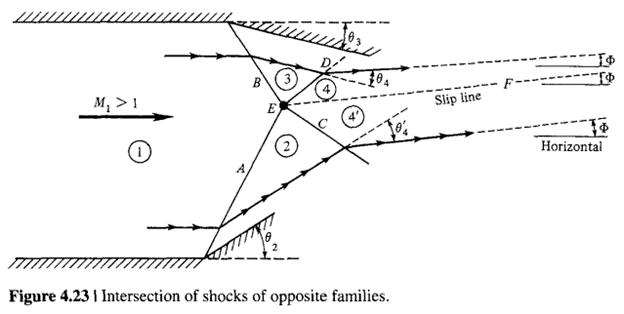
\includegraphics[scale=0.8]{../../images/problem_3/intersection_setup}
    \caption{Shock interaction problem setup}
    \label{shock_setup}
\end{figure}

\givens{}
\(M_1 = 3\)\\
\(p_1 = 1\,\unit{atm}\)\\
\(\theta_2 = 20^\circ\)\\
\(\theta_3 = 15^\circ\)\\

\assumptions{}

Flow in the duct will be considered inviscid, steady, and isentropic outside of the shocks.
In each region (1, 2, 3, 4, 4'), flow properties are constant and uniform, only changing across the shocks (A, B, C, D).
Changes in area are neglected.
There is no heat or work entering/exiting the system.
Flow in regions 4 and 4' are oriented in the same direction at an angle \(\Phi\) from the horizontal, with \(p_4 = p_{4'}\).
\(\Phi = \theta_3 + \theta_4 = \theta_2 + \theta_{4'}\).


\solution{}
\textit{Note: All calulations performed in MATLAB, see appendix \ref{Problem3MATLAB}.}\\
Given \(M_1\) and the two ramp angles, \(\theta_2\) and \(\theta_3\), shock angles \(\beta_2\) and \(\beta_3\) are found via the following relation using a numerical solver:

\[
    \tan{\theta_2}
    =
    2 \cot{\beta_2}
    \left[{
    \frac{M_1^2\sin^2{\beta_2}-1}{M_1^2\left({\gamma+\cos{2\beta_2}}\right)+2}
    }\right]
\]

\[
    \tan{\theta_3}
    =
    2 \cot{\beta_3}
    \left[{
    \frac{M_1^2\sin^2{\beta_3}-1}{M_1^2\left({\gamma+\cos{2\beta_3}}\right)+2}
    }\right]
\]

\[
    \boxed{
    \beta_2 = 37.7636^\circ \quad\quad \beta_3 = 32.2404^\circ
    }
\]

Post-oblique shock Mach numbers are calculated using the component of \(M_1\) normal to shock A and shock B, denoted by \(M_{1n,2}\) and \(M_{1n,3}\), respectively:

\[
    M_{1n,2} = M_1 \sin{\beta_2}
\]

\[
    M_{1n,3} = M_1 \sin{\beta_3}
\]

\[
    M_{2n}^2
    =
    \frac{M_{1n,2}^2 + \frac{2}{\gamma-1}}{\frac{2\gamma}{\gamma-1}M_{1n,2}^2-1}
\]

\[
    M_{3n}^2
    =
    \frac{M_{1n,3}^2 + \frac{2}{\gamma-1}}{\frac{2\gamma}{\gamma-1}M_{1n,3}^2-1}
\]

\[
    M_2 = \frac{M_{2n}}{\beta_2-\theta_2}
\]

\[
    M_3 = \frac{M_{3n}}{\beta_3-\theta_3}
\]

\[
    \boxed{
    M_2 = 1.9941 \quad\quad M_3 = 2.2549
    }
\]

Static pressure ratios across shocks A and B are found using oblique shock relations with \(M_1\) and the shock angles:  

\[
    \frac{p_2}{p_1}
    =
    1 + \frac{2}{\gamma+1}
    \left({
    M_1^2 \sin^2{\beta_2} - 1
    }\right)
\]

\[
    \frac{p_3}{p_1}
    =
    1 + \frac{2}{\gamma+1}
    \left({
    M_1^2 \sin^2{\beta_3} - 1
    }\right)
\]

\[
    \boxed{
    p_2 = 3.7713 \, \unit{atm} \quad\quad p_3 = 2.8216 \, \unit{atm}  
    }
\]

Solving for the conditions in regions 2 and 3 is a relatively trivial procedure.
In order to solve for the conditions in regions 4 and 4', an iterative approach must be used.
There are 5 unknowns needed to fully solve for the downstream conditions: \(\theta_4\), \(\theta_{4'}\), \(\beta_4\), \(\beta_{4'}\) and \(p_4\).
The corresponding equations used to solve for state 4 and 4':

\begin{itemize}

    \item Static pressure ratio across an oblique shock given that \(p_4 = p_{4'}\):

\[
    \frac{p_4}{p_3}
    =
    1 + \frac{2}{\gamma+1}
    \left({
    M_3^2 \sin^2{\beta_4} - 1
    }\right)
\]

\[
    \frac{p_{4}}{p_2}
    =
    1 + \frac{2}{\gamma+1}
    \left({
    M_2^2 \sin^2{\beta_{4'}} - 1
    }\right)
\]

\item \(\theta-\beta-\textrm{Mach}\) relations:

\[
    \tan{\theta_4}
    =
    2 \cot{\beta_4}
    \left[{
    \frac{M_3^2\sin^2{\beta_4}-1}{M_3^2\left({\gamma+\cos{2\beta_4}}\right)+2}
    }\right]
\]

\[
    \tan{\theta_{4'}}
    =
    2 \cot{\beta_{4'}}
    \left[{
    \frac{M_2^2\sin^2{\beta_{4'}}-1}{M_2^2\left({\gamma+\cos{2\beta_{4'}}}\right)+2}
    }\right]
\]

\item The objective function that will be used as a constraint is the relation between turn angles and \(\Phi\):

\[
    \Phi_4 =  \theta_3  + \theta_4
\]

\[
    \Phi_{4'} = \theta_2 + \theta_{4'}  
\]

\[
    \boxed{
    \theta_4  - \theta_{4'} + \theta_3 - \theta_2 = 0
    }
\]

\end{itemize}

The solution technique utilized to determine the correct downstream conditions is know as the secant method and is outlined below:

\begin{itemize}

\item Given two points, \((x_a,y_a)\) and \((x_b,y_b)\), the equation for a line connecting these points is given by point slope formula:

\[
    m = \frac{y_b-y_a}{x_b-x_a}
\]

\[
    y - y_0 = m(x-x_0)
\]

\item Let \((x_0,y_0) = (x_b,y_b)\):

\[
    y - y_b = \frac{y_b-y_a}{x_b-x_a} \left({x-x_b}\right)
\]

\item Plug in \(y=0\) to solve for the x-intercept of the line:

\[
    - y_b = \frac{y_b-y_a}{x_b-x_a} \left({x-x_b}\right)
\]

\[
    x = x_b - y_b\frac{y_b-y_a}{x_b-x_a}
\]

\item For an iterative solver this scheme becomes the following, known as secant method:

\[
    x_{i+1}= x_i - y_i\frac{y_i-y_{i-1}}{x_i-x_{i-1}}
\]

\end{itemize}

This method has the advantage of not needing to bound the true value of zero or determine if the sign of \(y_i\) changes relative to \(y_{i-1}\).
The solution method will involve iterating across values of downstream pressure, \(p_4\), calculating the value of the objective function, and iterating until the value converges to 0 within a chosen tolerance.
To better set up the initial conditions, values of the objective function are calculated until a sign change is observed, indicating that the zero lies between the previous two calculated points.
Figure \ref{obj_vs_p} shows the objective function versus \(p_4\) plotted to the point of the sign change.
The final two values of \(p_4\) will be used as the points \(x_1\) and \(x_2\) to initialize the secant method algorithm.

\newpage

\begin{figure}[h!]
    \centering
    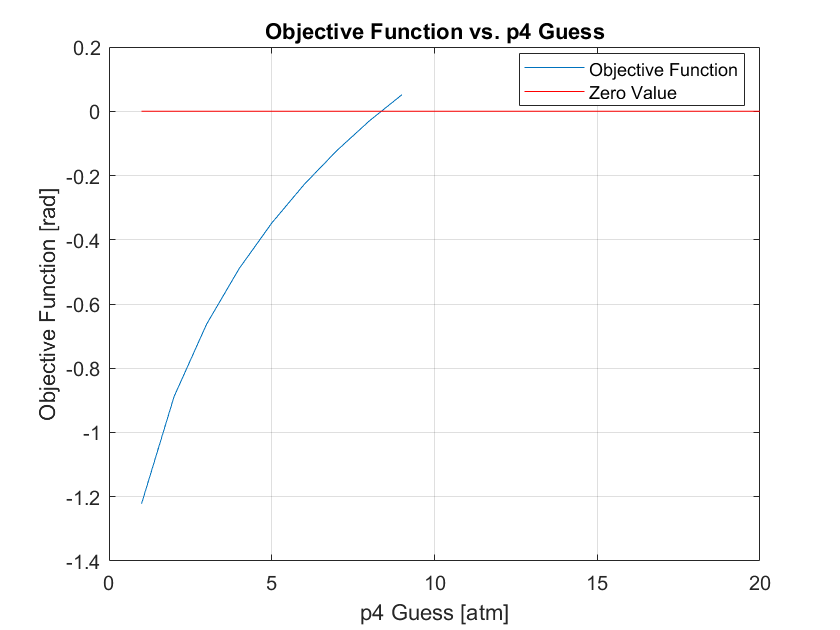
\includegraphics[scale=0.8]{../../images/problem_3/obj_vs_guess.png}
    \caption{Objective function value plotted against \(p_4\) guess to find sign change}
    \label{obj_vs_p}
\end{figure}

The secant method converges to an objective function value of 0 (tolerance = \(\num{1e-10}\)) in 6 iterations, yielding the following values for the unkown variables:

\[
    \boxed{
        \theta_4  - \theta_{4'} + \theta_3 - \theta_2 = 0
    }
\]

\[
    \boxed{
        p_4 = 8.3526\,\unit{atm}
    }
\]

\[
    \boxed{
        \theta_4 = 19.80^\circ
    }
\]

\[
    \boxed{
        \theta_{4'} = -15.20^\circ
    }
\]

\[
    \boxed{
        \Phi = 4.80^\circ
    }
\]

\[
    \boxed{
        \beta_4 = 46.55^\circ
    }
\]

\[
    \boxed{
        \beta_{4'} = -45.76^\circ
    }
\]

\end{document}
